\documentclass[11pt, twoside, twocolumn]{extarticle}
%\usepackage[showframe]{geometry}
\usepackage{graphicx}
\usepackage[utf8]{inputenc}
\usepackage{caption}
\usepackage{multicol}
\usepackage[toc, page]{appendix}
\usepackage{pgfplots}
\usepackage{subcaption}
\usepackage{listings}
\usepackage{hyperref}

\pgfplotsset{width=9cm,compat=1.9}
%\usepgfplotslibrary{external}
%\tikzexternalize
\usepackage[export]{adjustbox}
\usepackage[margin=0.5in]{geometry}
\PassOptionsToPackage{hyphens}{url}\usepackage{hyperref}
\usepackage{url}
\usepackage{import}
\usepackage{float}
\usepackage{listings}
\usepackage{color}
 
\definecolor{codegreen}{rgb}{0,0.6,0}
\definecolor{codegray}{rgb}{0.5,0.5,0.5}
\definecolor{codepurple}{rgb}{0.58,0,0.82}
\definecolor{backcolour}{rgb}{0.95,0.95,0.92}
\lstdefinestyle{mystyle}{
    backgroundcolor=\color{backcolour},   
    commentstyle=\color{codegreen},
    keywordstyle=\color{magenta},
    numberstyle=\tiny\color{codegray},
    stringstyle=\color{codepurple},
    basicstyle=\footnotesize,
    breakatwhitespace=false,         
    breaklines=true,                 
    captionpos=b,                    
    keepspaces=true,                 
    numbers=left,                    
    numbersep=5pt,                  
    showspaces=false,                
    showstringspaces=false,
    showtabs=false,                  
    tabsize=2
}
\lstset{style=mystyle} 
\usepackage{algorithm,algcompatible,amsmath}
\DeclareMathOperator*{\argmax}{\arg\!\max}% %https://tex.stackexchange.com/q/83169/5764
\algnewcommand\INPUT{\item[\textbf{Input:}]}%
\algnewcommand\OUTPUT{\item[\textbf{Output:}]}%


\usepackage[backend=bibtex, style=numeric, citestyle=numeric, url=true, hyperref=true]{biblatex}
\addbibresource{bibliography.bib}

\hypersetup{
    colorlinks=true,
    linkcolor=blue,
    filecolor=magenta,      
    urlcolor=cyan,
}

\title{\textbf{Implementing Critical Path Tracing: A Practitioner’s Approach}}
\date{}
\author{Robert McCartney, Bhavika Pravin Jain, Mohan Rao Divate Kodandarama\\
\small{\{mccartney, bhavikaj, mdivatek\}@stanford.edu} \\
Stanford University}

\begin{document}

\maketitle

\begin{abstract}
Modern day distributed systems are extremely complex deployments that constantly evolve in their features and data flows. A system like Google Search is going to have many separate teams of engineers working concurrently on the serving stack, with many downstream RPC calls and processing steps for each query. The latency characteristics of these systems can evolve rapidly, such as changing load from new emerging traffic patterns or new datacenter deployments.  Thus, keeping the latency of such a rapidly evolving system to a minimum is a challenging task.  Several existing techniques, including distributed tracing, CPU profiling, and RPC telemetry, all fall short of giving maintainers the information they need to know to fix latency regressions in practice.  

Taking a recently published ACM Queue article on Critical Path Tracing\cite{10.1145/3526967} (CPT), we use their techniques to implement a profiler that illuminates the root causes of system response time by identifying those subcomponents on the critical path contributing to overall latency.  This is done by first locally determining the critical path through a process's Java Dagger/Producers asynchronous programming framework and then aggregating these local paths across RPC boundaries, utilizing gRPC headers to propagate the path information for any given service specification.  This critical path tracing thus provides detailed and actionable information to maintainers about which modules of a large and complex distributed system are most culpable for its overall latency, so that optimizing them has a direct impact on system performance.

\end{abstract}

\section{Introduction}
Low latency is an essential feature for many online services.  As new features, functionality, and data flows are added to complex systems, keeping the overall latency to a minimum becomes challenging, as the root cause of any change in performance is often non-obvious. The goal of this project is to answer a key question, namely given a distributed system and workload, what subcomponents can be optimized to reduce end-to-end latency? 
Critical path tracing is a new applied mechanism for gathering latency profiles at scale in large distributed applications\cite{10.1145/3526967}. It provides detailed and actionable information for maintainers looking to reduce latency or discover the source of a recent regression.  A \textit{critical path} describes the single sequence of dependent steps that form the slowest path of a processed request, such that optimizing any of these steps reduces the overall latency. Thus, a critical path is the longest single duration of processing steps, both within and between processes, that form a dependency chain.  If the entire distributed system is viewed as a large, directed execution graph with latency labels at each node, the critical path is a directed walk through the graph that maximizes the sum of node latencies.  

Large Web applications typically consist of many separate services, and CPT relies on application programmers using server frameworks to instrument each of these subcomponents.  This allows for the logic that propagates and aggregates critical paths to be built into the framework, so no incremental work is necessary to start passing critical paths among callers and callees built and maintained by different engineering teams.  Specifically, when one microservice (the client) calls another (the server), the critical path information from the server is returned back to the client via the remote procedure call (RPC) metadata, so it never appears within any application-layer service definition.  The caller may in fact also be a server to some other client upstream of it, and thus must merge the information from all its downstream dependencies into a unified critical path for that specific request execution. In the original paper, the top level service finished by logging this unified critical path for the entire request, to be consumed later for use in statistical analysis and A/B experimentation frameworks.  Their log analysis can create `average' RPC profiles by aggregating over many similar request types.  Here, we instead extend their approach to include a frontend for realtime analysis of each request's critical path as it occurs.  We also utilize the open source gRPC framework for distributed communication, rather than the proprietary Google channels used in the paper.

The process of CPT is very efficient compared to traditional distributed tracing, as each subcomponent is pruning a complex execution graph down to a single linear one, by recursively combining the linear paths of its dependencies and of its own internal processing. This enables a large number of requests to be sampled, and the resulting profiles give actionable, fine-grained coverage of distributed sources of latency.

\section{Related Approaches}

There are some well known existing techniques for monitoring the latency of distributed systems today, with the most common techniques of RPC telemetry, CPU profiling, and distributed tracing in use for most major, large scale deployments.

\subsection{RPC Telemetry}
In this technique, services export individual RPC-level information, such as how many times a remote procedure call is made to the service, its error rate and latency, and any slices of interest. Monitoring services collect and display this information on dashboards or persist it in logs. This approach works well when there are only a few RPC calls that are critical for overall service latency, such that any change in that RPC directly impacts the overall service's latency metric. However, this approach struggles in some common scenarios - 
    \begin{itemize}
    \item Multiple RPCs. When a service calls multiple other services asynchronously or repeatedly, the relationship between them matters.
    \item Heterogeneous  workloads. Since the exported metrics of the RPC are averaged over multiple requests, the latency information about low frequency requests or particular request types may be lost.
    \item Causality. Even if a given RPC call increases in latency, it might not be the cause of the overall service degradation, if for instance some other increase in cpu-bound work happened to occur at the same time.  
    \end{itemize}
    
\subsection{CPU Profiling}
CPU Profilers work well if you already know an expensive subcomponent that needs to be optimized.  Function call stacks along with CPU samples are collected to provide insights into expensive code paths.  Thus you can get in-depth insight into lock contentions, disk accesses, or other sources of latency for any component.  However, they do not track latency across RPC boundaries, and if you are optimizing a module that is off the critical path it could have no impact on overall service latency.  In some respects, profiling should be considered complementary to CPT, since once an expensive method is identified by CPT, CPU profiling can be used to dig deeper into its stack frames.

\subsection{Distributed Tracing}
In this approach, the entire flow of control through the distributed system is tracked, with timing points and additional data captured for analysis\cite{36356}.  Unlike RPC telemetry, distributed tracing can make sense of parallelism and heterogeneous workloads since the information about external service requests and their latency is collected.  However, these traces are often expensive, causing in practice only a small sample of all requests to be traced.  Depending on the system, you often also need to manually annotate those portions of the code to trace, and may need to join across service logs to recreate the full trace, which can be an expensive operation.  CPT overcomes these limitation by only keeping a small subset of the entire trace, namely that portion on the critical path, and passing it via RPC metadata for collection, logging, and analysis at the top level service. In the evaluation section below we compare our implementation of CPT to the PerfMark distributed tracing library\cite{PerfMark}, which is a manually instrumented tracing library for Java. 

\section{Challenges and Motivation}

Most of the commonly used latency analysis tools have at least one of the following limitations, which we set out to overcome by applying the techniques first popularized within Google Search as described in \cite{10.1145/3526967}.

\begin{itemize}
    \item Able to measure only one component, not end-to-end latency
    \item Struggle to make sense of parallelism between services and how internal processing interacts with asynchronous calls
    \item Struggle to make sense of repeated RPC calls and data dependencies during execution
    \item Show inflexible approaches to providing dimensional slices
    \item Require additional complex analysis on top of the collected data to identify root causes of latency for the overall system
    \item Have difficulty handling heterogeneous workloads and present information gaps around low-volume requests
\end{itemize}

CPT addresses the above limitations.  It can be thought of as part CPU profiling, by surfacing method-level metrics; part RPC telemetry, by surfacing RPC latencies; and part distributed tracing, by following one request through its full distributed execution. It can do these things at a fraction of the cost of traditional distributed tracing, since the return value at each service is a single list of \lstinline|{Component, Cost}| pairs, with recursive list merging occurring upon the conclusion of processing at each node.  The final output is a fraction of the total execution path of the full distributed trace, and CPT can calculate this path without needing any special code instrumentation.

\section{Tech Stack and Architecture}

\subsubsection*{Libraries}

\textbf{Protocol Buffers:} Protocol buffers\cite{protobuff} are a language-neutral, platform-neutral, extensible mechanism for serializing structured data. Like \lstinline{JSON} it can be used to pass messages between services, but the wire format of the serialized data is much more packed (and as a result non-human readable) for greater network utilization. The user defines the structure of data, from which the proto compiler generates the source code to read and write to the data streams.  In our case, we used the Java version of the proto compiler.

\textbf{gRPC:} Written on top of protocol buffers, gRPC\cite{grpc} is an open-source RPC framework designed by Google to achieve high-speed communication between microservices. It allows developers to integrate services programmed in different languages. gRPC passes serialized data on top of the HTTP/2 protocol, while gRPC-Web uses HTTP/1 since HTTP/2 is not yet supported by many browsers. Using gRPC, a client can directly call a method on a remote server as if it were a local object.  As in many RPC systems, gRPC is based around the idea of defining a service separate from its implementation, by specifying its parameters and return types. The server implements this interface and runs gRPC to route client calls to its implementation. The client links against a stub that appears to the application as a local method call. gRPC is roughly 7 times faster than REST due to the use of Protocol Buffers and HTTP/2\cite{gRPCvsREST}.

\textbf{Dagger:} Dagger\cite{dagger} is a compile-time framework for dependency injection. Compared to other dependency frameworks such as Spring and Guice that use reflection for dependency injection during application execution, Dagger plugs itself into the Java compilation workflow and generates static code to resolve requested object dependencies. This means there is no runtime overhead, making it more suitable for embedded and native applications where reflection is too expensive, and the generated source code pushes many programming mistakes from runtime into compile-time, making debugging easier and safer.

\textbf{Dagger Producers:} Dagger Producers\cite{daggerproducers} is an extension to Dagger that utilizes its graph-based dependency injection framework as an asynchronous programming paradigm in Java. It lets you code synchronous methods, with the output of each method being a \lstinline{ListenableFuture} representing some asynchronous return value from the computation.  The framework takes care of scheduling each method as its required inputs become available, creating a ``computation graph" to execute via a user-supplied \lstinline{Executor} - in essence a graph of computation dependencies rather than synchronous object dependencies.  In many ways it mirrors an event-driven architecture, as opposed to a thread-based one \cite{threadbad}.  Understanding the control flow and path through the computation graph is one commonly known issue that arises under this approach \cite{270302}.

\textbf{D3.js:} D3.js\cite{d3js} (also known as Data-Driven Documents) is a JavaScript library for creating dynamic, interactive data visualizations in the web browser.  D3 allows you to bind arbitrary data to the Document Object Model (DOM), and then apply data-driven transformations to the document. We utilize this library to visualize the critical path data, giving real time insights into the dynamic application data and helping the user to inspect latency causality.

\subsubsection*{Backend}

\begin{figure}[h]
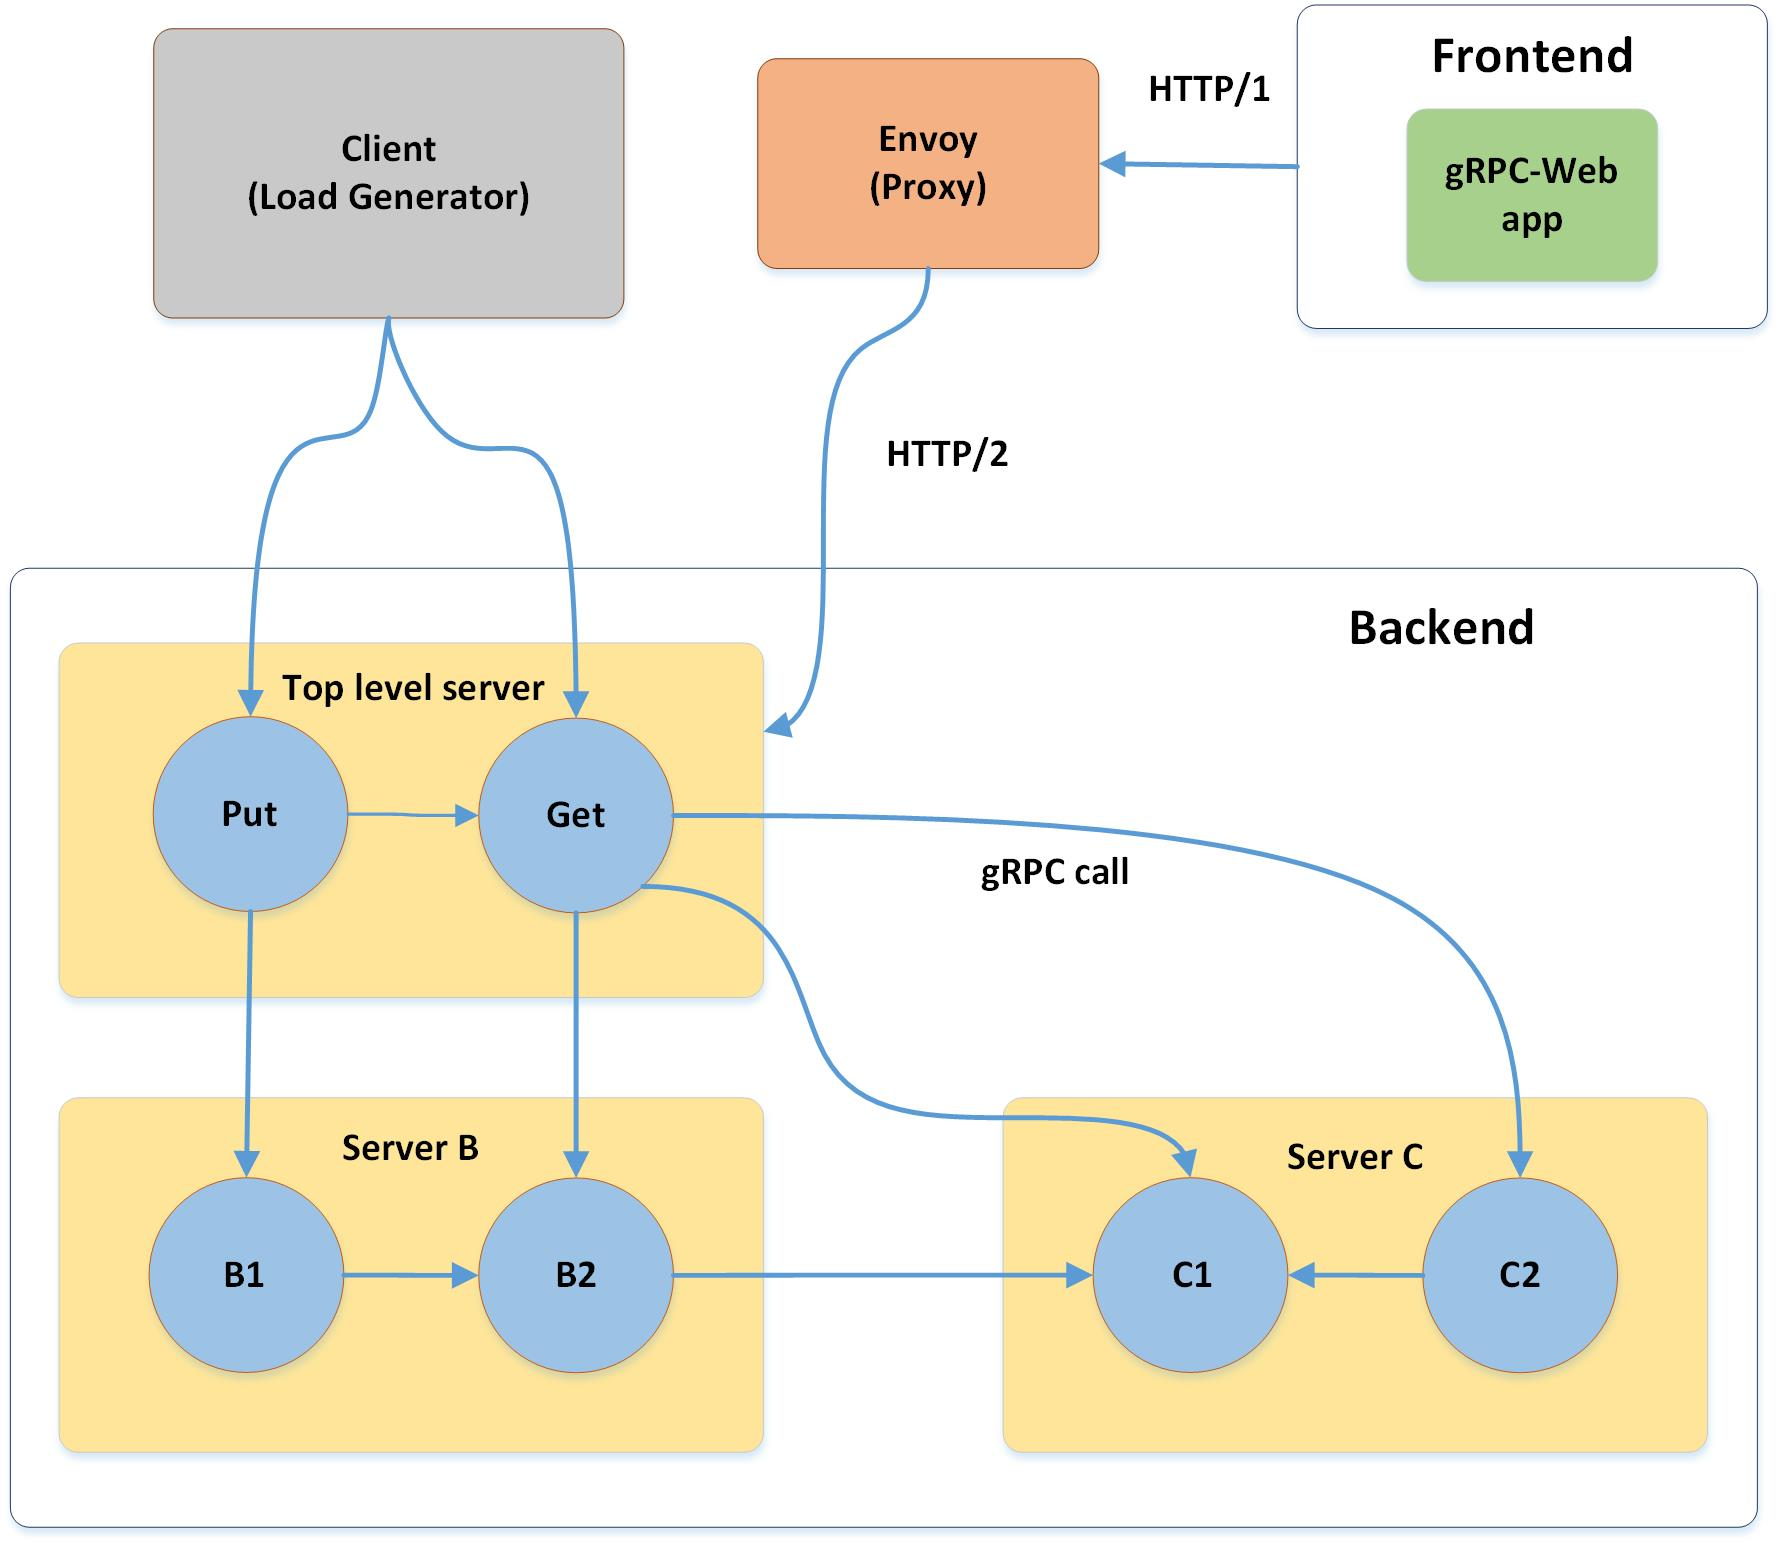
\includegraphics[width=\linewidth]{architecture.jpg}
\caption{Architecture}
\label{fig:architecture}
\end{figure}

Our distributed system consists of three servers, which we named \lstinline{TopLevelServer}, \lstinline{ServerB}, and \lstinline{ServerC}. We used the Dagger/Producers framework to internally implement the asynchronous processing inside each server, and used gRPC to communicate between servers.  As seen in Figure \ref{fig:architecture}, the \lstinline{TopLevelServer} implements \textit{Get(String)} and \textit{Put(String, String)} requests, with the dependencies between the servers mirroring those in \cite{10.1145/3526967}.  The implementations are such that certain requests will conditionally execute the Producer graph in different orders, such as changing RPCs from parallel to serial to represent data dependencies and heterogeneous workloads. We also conditionally made some of the service methods sleep for varying lengths to simulate different cpu-bound workloads.

\subsubsection*{Frontend}

As shown in Figure \ref{fig:architecture}, the Web app utilizes gRPC-Web, which allows a single protocol buffer service definition to be shared between both the frontend and backend servers.  This is much more convenient than a separate REST/JSON frontend serice that needs middleware to translate into backend protocol buffers.  However, this approach does necessitate the use of \textit{Envoy Proxy}\cite{envoyproxy}, which has built-in support for gRPC-Web and serves as its default service gateway.  This additional service is launched via Docker to translate HTTP/1.1 to HTTP/2 calls as the Web app communicates with the \lstinline{TopLevelServer}.  The actual HTML is served via the small Python \lstinline{http.server}, with Node.js\cite{Nodejs} used for the JavaScript runtime environment.  In addition, the D3.js library\cite{d3js} is used to visualize critical path information.

\section{Implementation}

The codebase is around 4k lines of code, and balloons to over 24k lines once all the code generation steps are run (Dagger, Producers, and Protoc). Originally when we chose the project, we thought that the statistics from Producer execution would be available as part of the framework, and that the compile-time constructed graph would be available and consumable.  However, we found on \url{https://dagger.dev/dev-guide/producers} the ominous warning: \textbf{As of March 2016, not implemented yet}. Thus, our first step was to instrument Producers to capture timing information.  Following that, we had to implement a distributed tracing ID, utilize both client and server RPC interceptors to pass metadata outside the scope of service definitions.  With that we could calculate critical paths, and recursively combine such paths using heuristics from other instrumentation.  The majority of this functionality is contained in the \lstinline{src/main/java/kvprog/common} directory.  In keeping with our goal to not need to instrument application code, the interceptor and timing logic can be added to any Dagger/Producers server by including \lstinline{InterceptorModule.class} into the top-level component for its global bindings and \lstinline{MonitorModule.class} into the ProductionComponent Producer Graph for the remaining call-scoped bindings.

\begin{figure}[h]
\centering
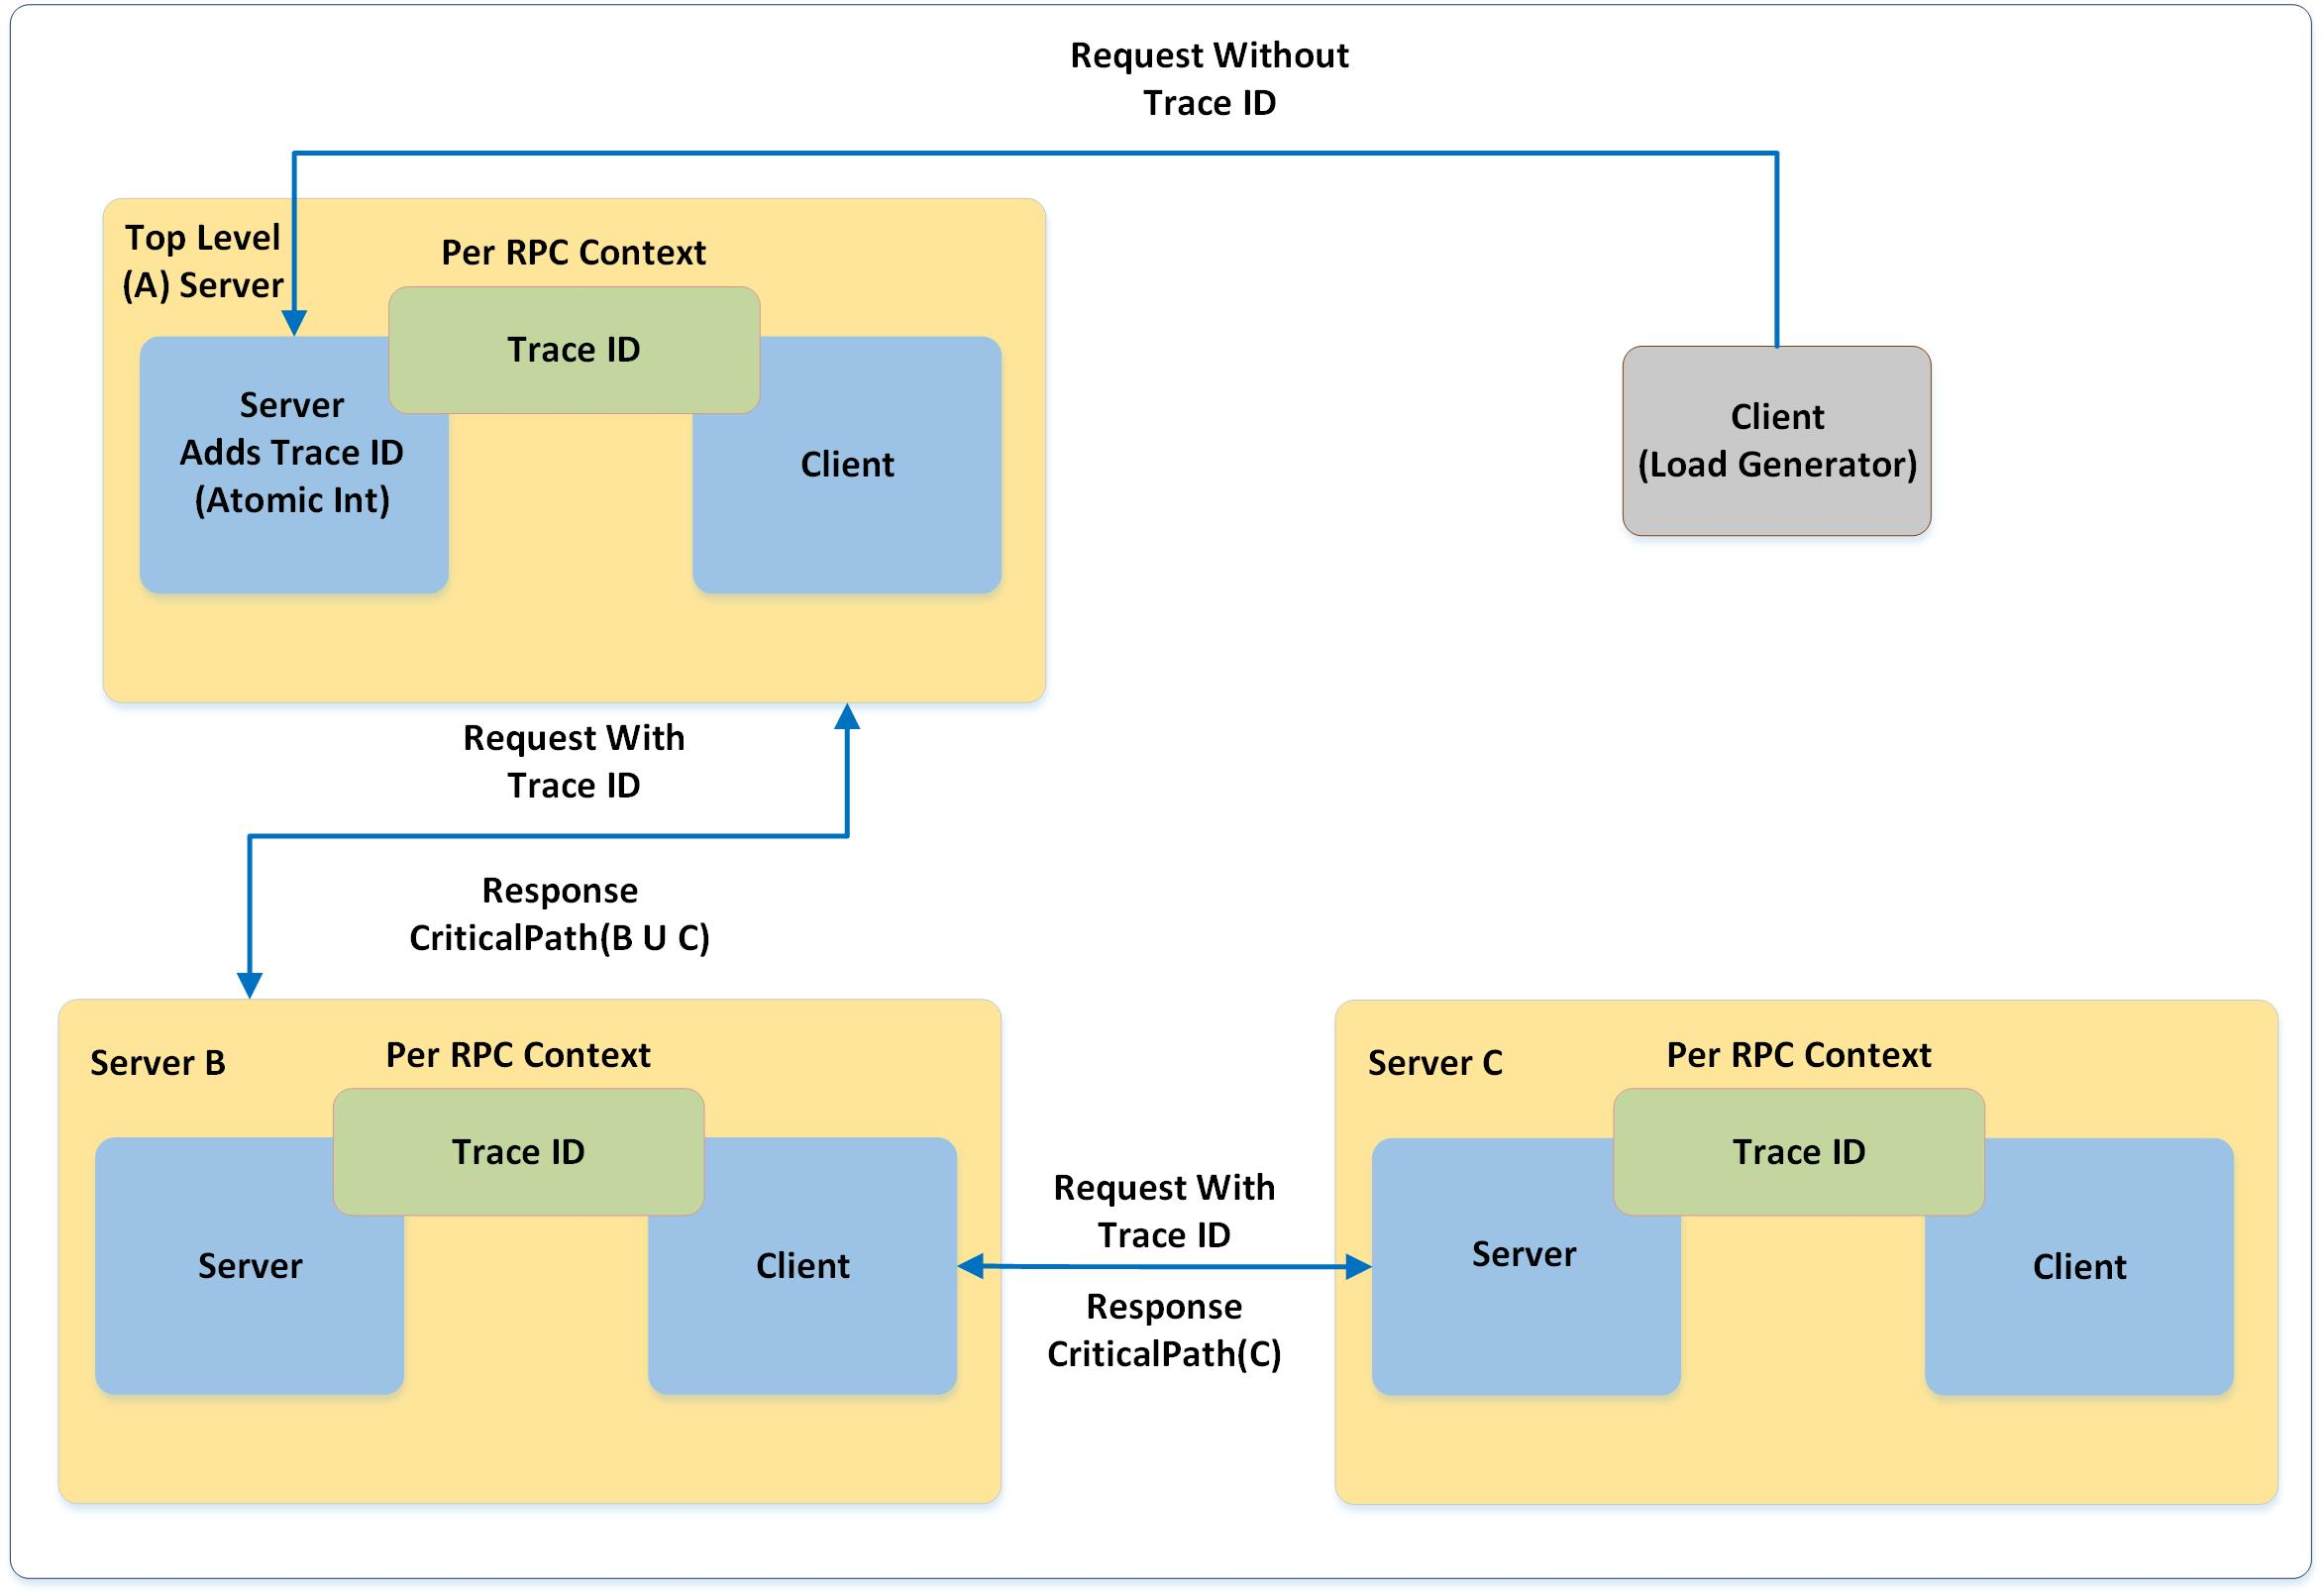
\includegraphics[width=\linewidth]{implementation.jpg}
\caption[width=\linewidth]{Implementation Details}
\label{implementation}
\end{figure}
    
\subsection{Instrumenting Time}

Producers exposes the \lstinline{ProductionComponentMonitor} interface to provide custom monitoring of Producer methods. It is created once per Producer graph, and is then asked to create \lstinline{ProducerMonitors} to hook into each method's lifecycle events. The events we utilized:
\begin{lstlisting}
    public void methodStarting();
    public void methodFinished();
    public void succeeded(Object o);
    public void failed(Throwable t);
\end{lstlisting}
Through this we can calculate the time taken in every method. Note that \lstinline{methodFinished} ends upon creation of the \lstinline{ListenableFuture}, so encapsulates CPU time taken, but for critical path computations we need to know when the actual Future completed to kick off whatever dependency waited for it, which is captured via the \lstinline{succeeded} event.

\subsection{Critical Path Computation}

In theory, since Dagger creates a static graph at compilation, we should be able to determine exactly what Producer method called another. We discuss such an approach in Section \ref{future}. Without that, we had to use heuristics to calculate the critical path. First, we captured the global execution ordering of each Producer method according to its start time, as it scheduled to run on one of the threads in the \lstinline{ExecutorService} threadpool. By knowing what Producer was currently scheduled on a \lstinline{ThreadLocal} when entering an RPC client interceptor, we can mark that method as making an external RPC call, and subdivide its timing information with the critical path returned from that call. At the end of the Producer graph execution, we then work backwards on the execution order list we created, constructing a critical path using the heuristic that either the local method or RPC call which completed most closely to start time of the current Node was what my Producer was waiting on.  This heuristic minimizes unaccounted for 'framework' time which would otherwise exist. In addition, RPCs are marked as occurring in parallel using a Cache on the \lstinline{trace_id}, where we decide that any RPC that started before another one finished is an independent path.

\subsection{Context and Metadata}

There still exists the issue of how to pass critical path information across RPC boundaries, and how to pass the \lstinline{trace_id} that correlates RPC calls as coming from the same top-level request. This is done through two properties of gRPC, the \lstinline{Context} and both request and response \lstinline{Metadata}.  Context is a per-request data structure provided by gRPC, where you can stick data associated to a key.  This allows for information sharing between the Server and Client RPC interceptors on a single service.  The top level server creates the initial \lstinline{trace_id} using an \lstinline{AtomicInt} and places it into the side-channel Metadata of the RPC call. Subsequent servers pull it out of Metadata and place it back into their local Context, where it can be further propagated by their own Client.  In the same way when returning calls back upstream, each critical path is inserted into the Metadata, which the client reads and parses to apply to its own children critical paths.

\section{Evaluation}

\begin{figure}[h]
\centering
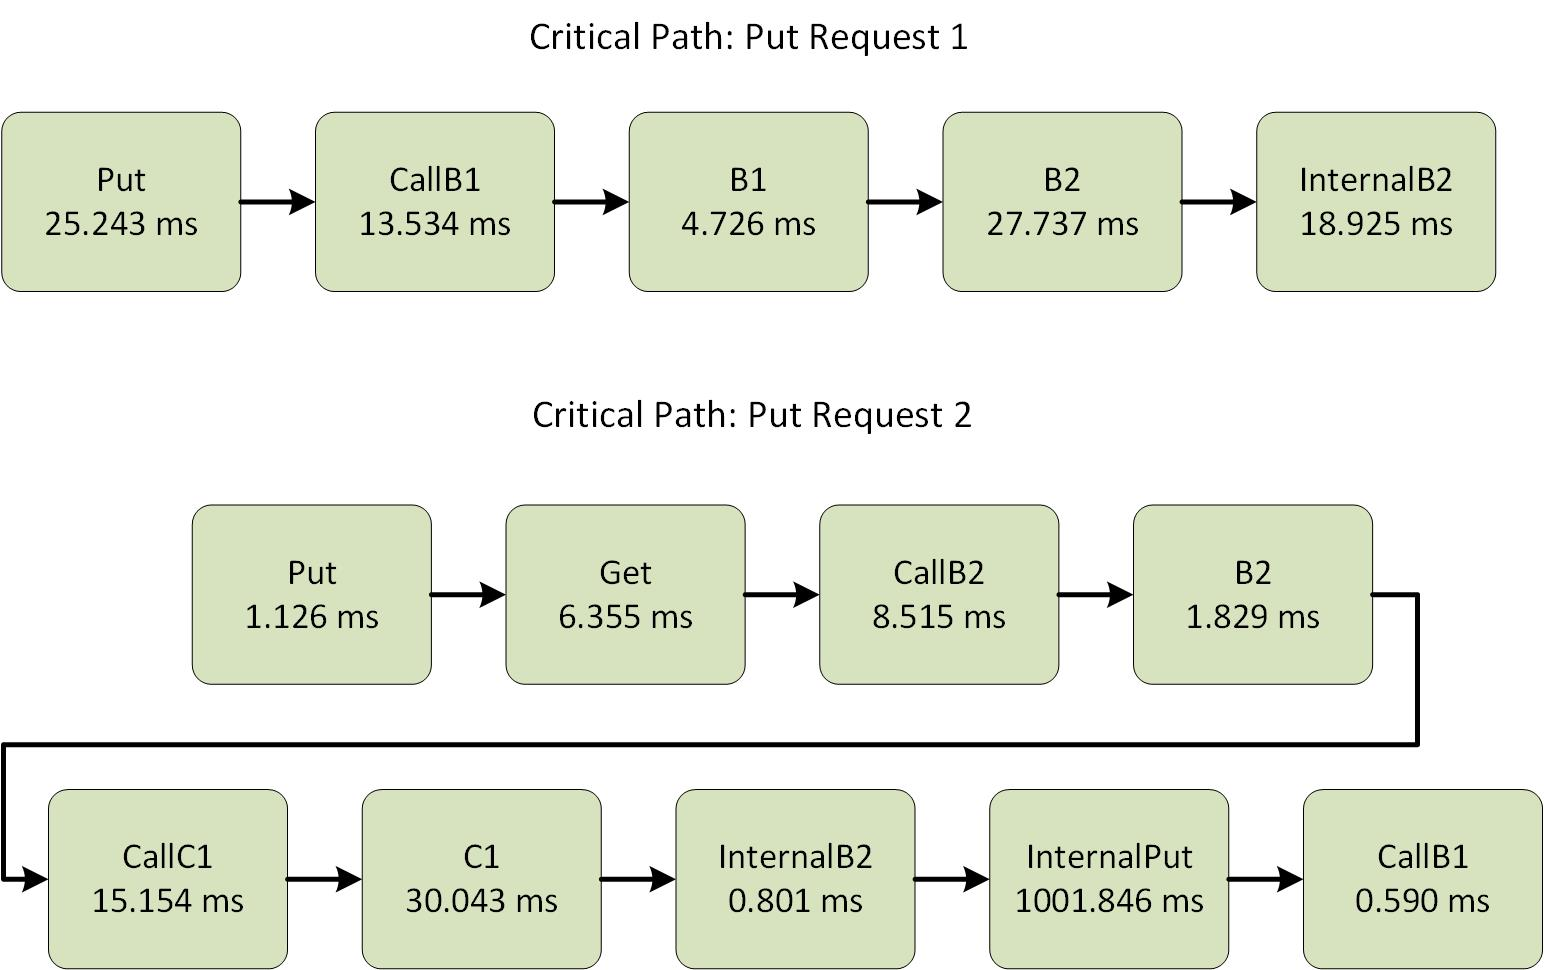
\includegraphics[width=\linewidth]{evaluation.jpg}
\caption[width=\linewidth]{Critcal paths for different Put requests}
\label{eval_put}
\end{figure}

Using our CPT framework and the test system from Figure \ref{fig:architecture}, we instrumented RPC calls to perform differently for different inputs and visualized the changes in the critical path produced. 

\subsubsection*{PUT}

As seen in Figure \ref{fig:architecture}, a Put request will call either B1 or Get (or both, as we cannot tell from this high level diagram). We implemented the call so that Get was only called conditionally, if the key passed in the request was \lstinline{queryOfDeath}. In this case we also sleep for 1 second to represent heavy cpu-bound processing.  In the first request of Figure \ref{eval_put}, you can see the critical path returned only makes a call to B1, which in turn calls the local B2 module.  However, in the second request we passed the \lstinline{queryOfDeath}, which exploded the critical path taken to include the conditional call to Get.  In addition, we see the 1 second delay on the \lstinline{InternalPut} processing stage.

\subsubsection*{GET}

\begin{figure}[h]
\centering
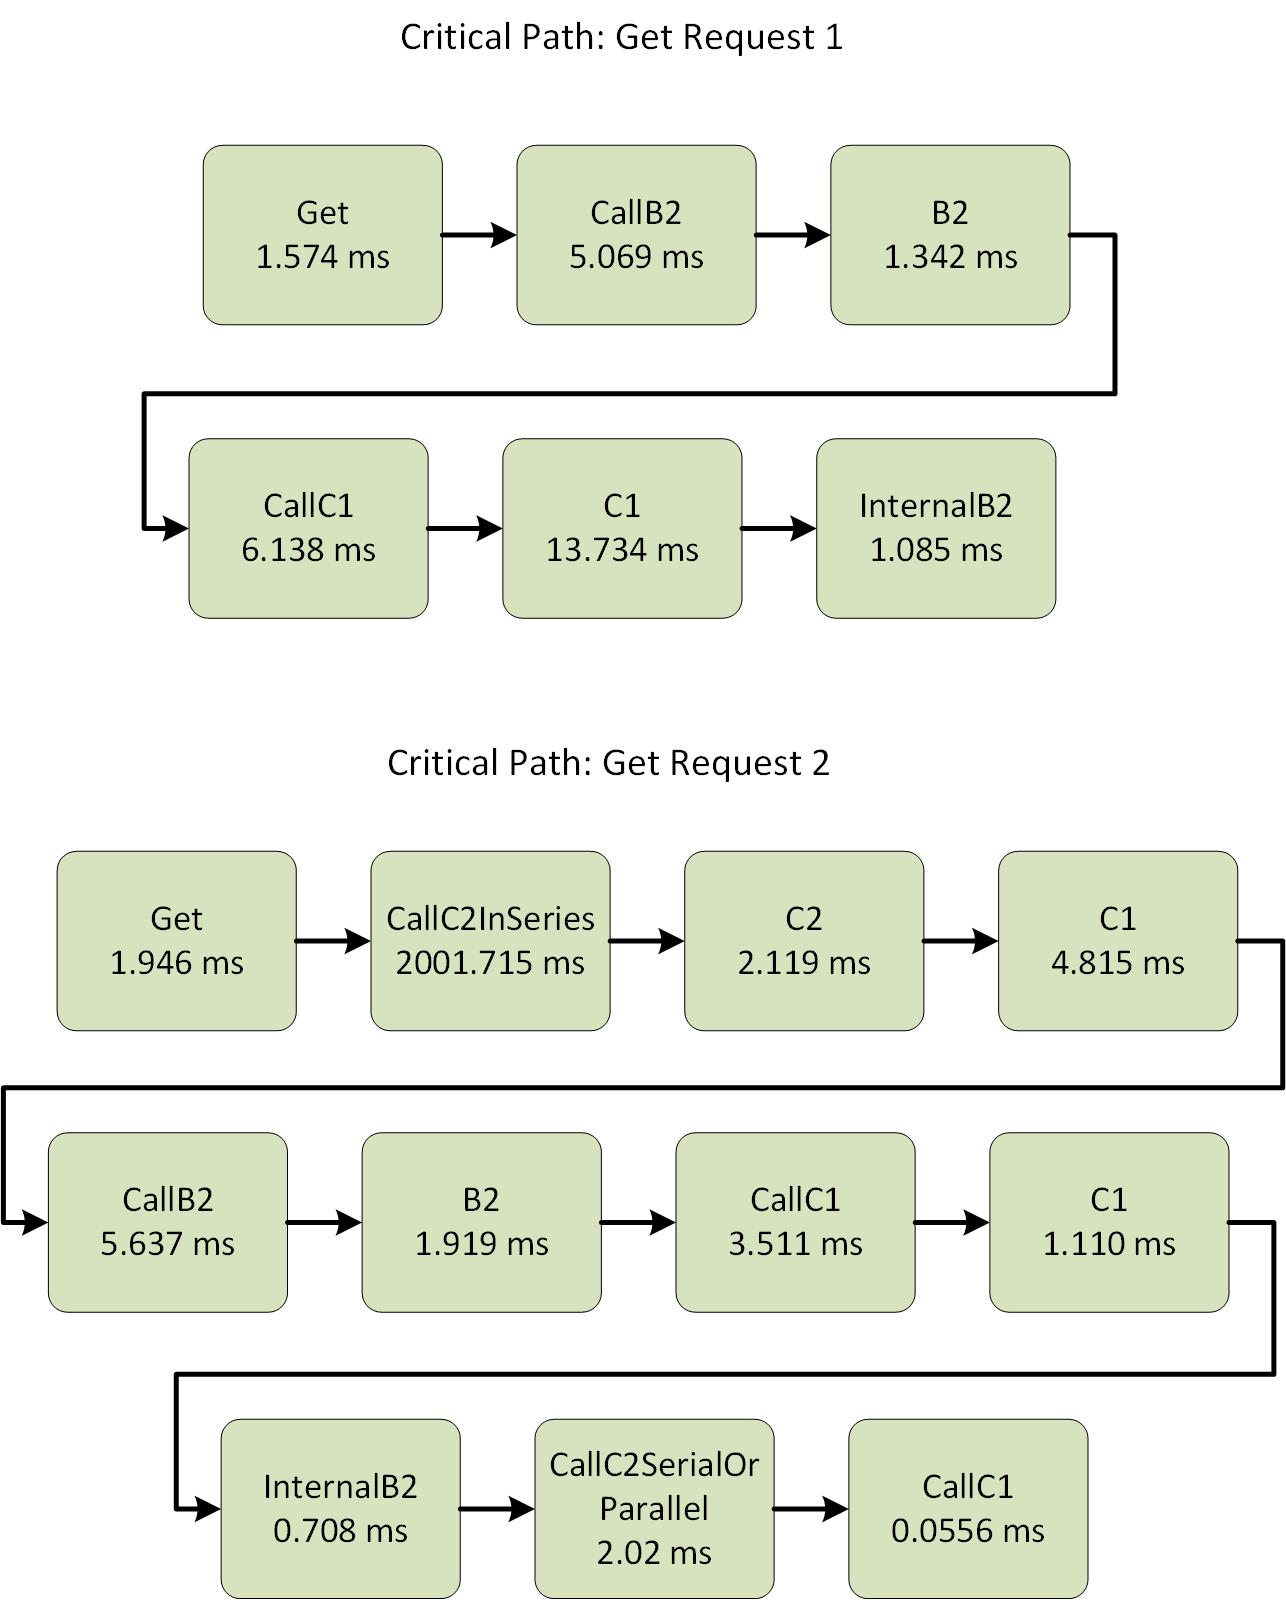
\includegraphics[width=\linewidth]{evaluation2.jpg}
\caption[width=\linewidth]{Critcal paths for different Get requests}
\label{eval_get}
\end{figure}

Figure \ref{eval_get} shows a second example of heterogenous RPC calls taking different critical paths.  Once again, the high level dependencies are showcased in Figure \ref{fig:architecture}, but the actual execution paths depend on the input key provided.  In this case, the special key \lstinline{CallC2InSeries} changes the parallel calls from Get to B2 and Get to C2 to instead be in series, mimicking a data dependency where the result of one RPC is needed to form the request of the follow-on RPC.  In the first request, the call to C2 is completed elided, which is expected as a single hop from \lstinline{TopLevelServer} to \lstinline{ServerC} should be lower latency than the two hops shown from \lstinline{TopLevelServer} to \lstinline{ServerB} to \lstinline{ServerC}.  In the second request, we see the large increase in the critical path from the in-series requests, as well as the 2 second sleep occurring on an internal processing step.  In a real world system, upon seeing this graph an engineer could investigate if this serial call was a misconfiguration or in fact working as intended.

\subsubsection*{PerfMark comparison}

\begin{figure}
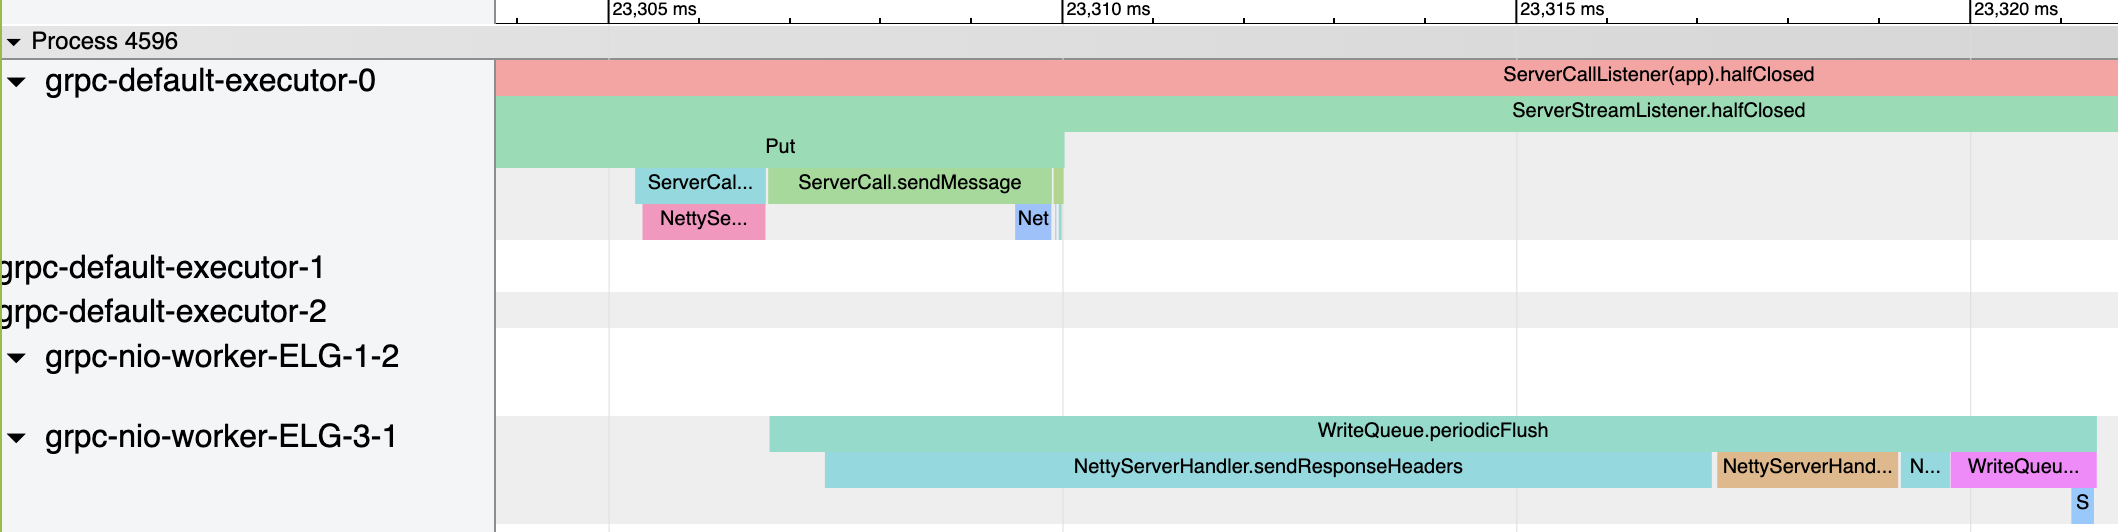
\includegraphics[width=\linewidth]{
PERFMARK_GRAPH}
\caption[width=\linewidth]{Perfmark-trace}
\label{perfmark}
\end{figure}

To highlight how CPT differs from other systems, we include in Figure \ref{perfmark} the output from a typical distributed trace. Such traces are indeed a wealth of information, giving extremely granular information on what computation each thread was performing for each unit of time.  However, it suffers from two critical shortfalls:

\begin{enumerate}
    \item We can see the highest latency segments, but there is no guarantee that optimizing those segments would reduce overall latency, if they are away from the critical path.
    \item To produce this graph, we had to manually instrument our code using code blocks like \lstinline{PerfMark.traceTask("Get")}, which is not scalable across a large distributed system in which we don't even maintain every subcomponent.
\end{enumerate}

\section{Shortfalls}

While a very useful approach, CPT does suffer from some shortfalls which should be recognized.  One is that you may still need more information after finding the critical path to actually optimize it.  Things like lock contention or slow disks would not be immediately clear, and likely need more in-depth CPU profiling to diagnose.  Another is that you could optimize the critical path only to have it then change, without a large latency improvement.  This is related to the concepts of drag and slack outlined in \cite{10.1145/3526967}. Finally, for large critical paths there is real network costs to passing the extra binary data around in HTTP headers.  This is typically mitigated through a sampling regime.

\section{Future Work}\label{future}

We did not have access to a static dependency graph, and thus had to use a heuristic to recreate the path of execution. The Dagger Service Provider Interface (SPI)\cite{daggerspi} is a mechanism to hook into Dagger’s annotation processor and access the binding graph model that Dagger creates during compilation. Using this framework, we could save the static graph to a proto and consume it into our critical path calculation at runtime. One example of SPI in action is shown in Figure \ref{fig:dependency_graph}, which is produced by the Scabbard\cite{scabbard} plugin to generate \lstinline{png} images of the dependency graph.

\begin{figure*}[h]
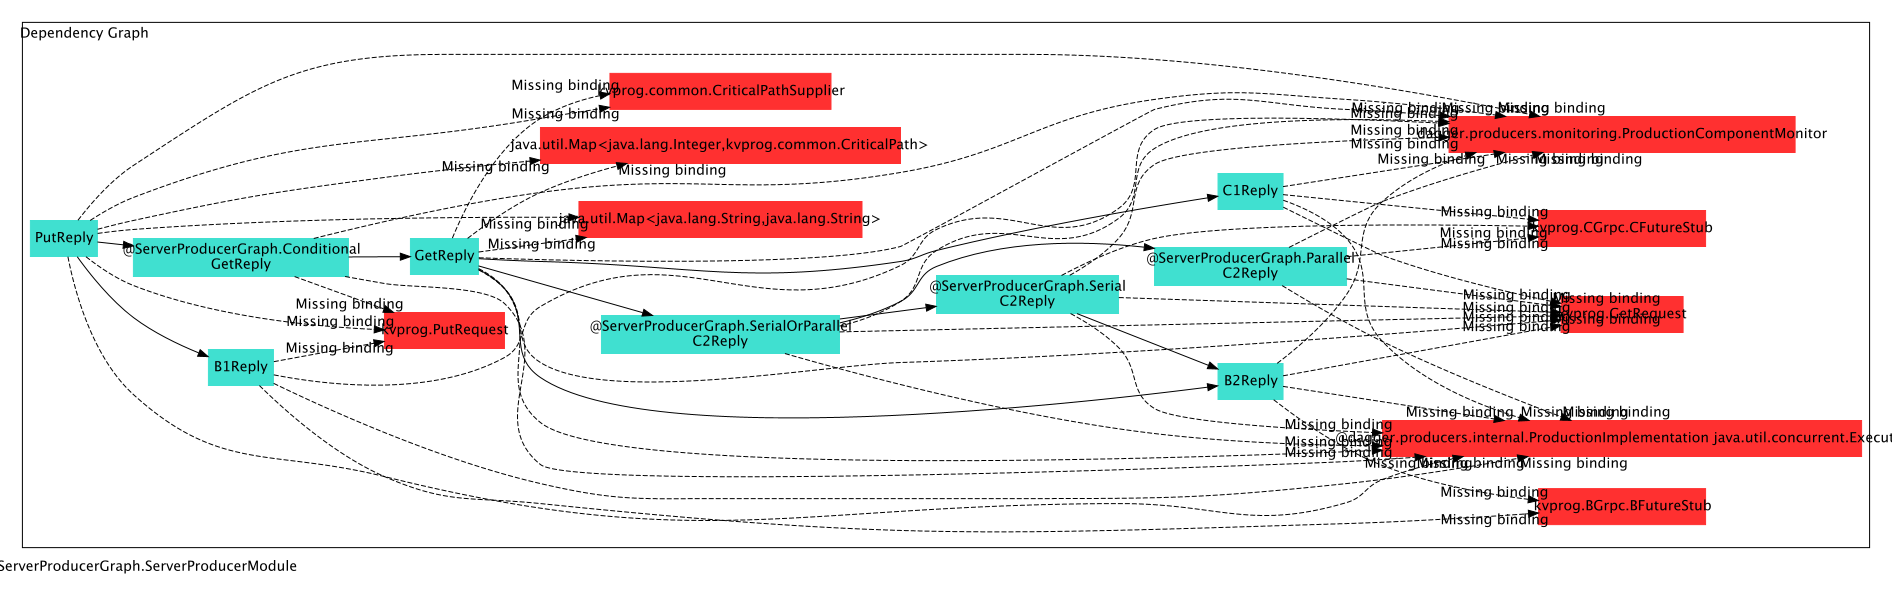
\includegraphics[width=\linewidth]{ServerProducerModule.png}
\caption[width=\linewidth, scale=1.5]{Dependency graph generated by Scabbard}
\label{fig:dependency_graph}
\end{figure*}

\section{Conclusion}

Critical path tracing addresses the limitations of other common latency analysis methods such as RPC telemetry, CPU profiling, and distributed tracing. In this work, we have demonstrated how CPT can be implemented for gRPC using Dagger/Producers.  Further, we have added to the original approach with a gRPC-Web frontend to display real time critical path information.

\section{Acknowledgements}
We would like to thank Eaton et al.\cite{10.1145/3526967} for creating Critical Path Tracing and Prof. David Mazières for his feedback on this practical implementation.

\printbibliography

\end{document}
 